%************************************************
\chapter{Draft}\label{ch:draft}
%************************************************


\section{Smart card APDU}

To communicate the smart cards and the reader an standardized protocol is specified in ISO/IEC 7816-4 \citep{APDUISO}.

The messages, also kown as \ac{APDU}, are divided in APDU Commands and APDU Responses.

\textbf{APDU Commands} consist in 4 mandatory bytes (CLA, INS, P1, P2), and an optional payload.

\begin{itemize}
	\item CLA byte: Instruction class. Denotes if the command is interindustry standard or proprietary.
	\item INS byte: Instruction code. Indicates the specific command.
	\item P1, P2 bytes: Instruction parameters.
	\item Lc, 0-3 bytes: Command data length.
	\item Command data: Lc bytes of data.
	\item Le, 0-3 bytes: Expected response data length.
\end{itemize}

This way, minimal number of bytes are needed to transmit commands to the smart card, allowing manufacturer's personalization of the smart card behavior and capabilities along with standard operations.

\begin{figure}[bth]
	\begin{center}
		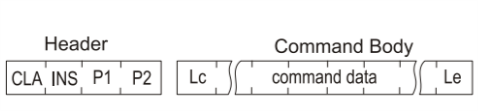
\includegraphics[width=0.55\linewidth]{gfx/APDUCommand}
	\end{center}
	\caption{APDU Command}
	\label{fig:APDUCommand}
\end{figure}


\textbf{APDU Responses} are generated inside the smart card, always as an answer to an APDU Command. They consist on an optional payload and two mandatory status bytes.


\begin{itemize}
	\item Response data: At most Le bytes of data.
	\item SW1-SW2 bytes: Status bytes. Encode the exit status of the instruction.
\end{itemize}

\begin{figure}[bth]
	\begin{center}
		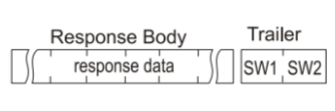
\includegraphics[width=0.55\linewidth]{gfx/APDUResponse}
	\end{center}
	\caption{APDU Response}
	\label{fig:APDUResponse}
\end{figure}




\hfil


The transmission protocol varies between different types of readers and smart cards (e.g. chip, contact-less), but what is common between every smart card interaction, is the \textit{APDU Command-Response Dialogue}. As long as the smart card has a power supply, it can maintain the dynamic memory in RAM between APDU Commands, what allows to do in two or more commmands complex operations, transmit more bytes than a single APDU can admit, etc.



\begin{figure}[bth]
	\begin{center}
		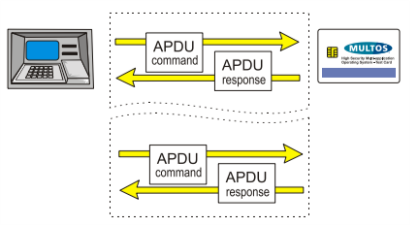
\includegraphics[width=0.75\linewidth]{gfx/APDUdialog}
	\end{center}
	\caption{APDU Command-Response Dialogue}
	\label{fig:APDUdialog}
\end{figure}



\section{P2ABCE}


In the \ac{P2ABCE} repository \citep{p2abcurl} is available the project's code, divided in two solutions: a complete P2ABCE implementation in Java and a Multos Smartcard implementation as companion for the project.

The Java code is managed by a Maven project, structured using various known design patterns, but not of our interest. The structure we are actually interested in are the REST Services and their use of the Components classes, in which the smartcards are included.

P2ABCE project is based on the concept of smartcards to store the credentials, logical or physical. An interface is defined to communicate with these smartcards, and then different implementations allow to use either \textit{Software Smartcards} or \textit{Hardware Smartcards}. 

The \textit{SoftwareSmartcard} class implements the interface in Java, suitable for tests and self-stored smartcards that any application using P2ABCE may need.

The \textit{HardwareSmartcard} class uses the standard APDU messages [TODO:ref] to interact with smartcards. P2ABCE defines for every method in the mentioned interface, the necessary APDU instructions, and currently relies on \textit{javax.smartcardio} abstract classes (implemented by Oracle in their JRE) to communicate with the smartcard reader. This way, it doesn't matter what manufacturer issues the smartcard, or if it's an Android device, if they support the APDU API, P2ABCE will work with them.

\begin{figure}[bth]
	\begin{center}
		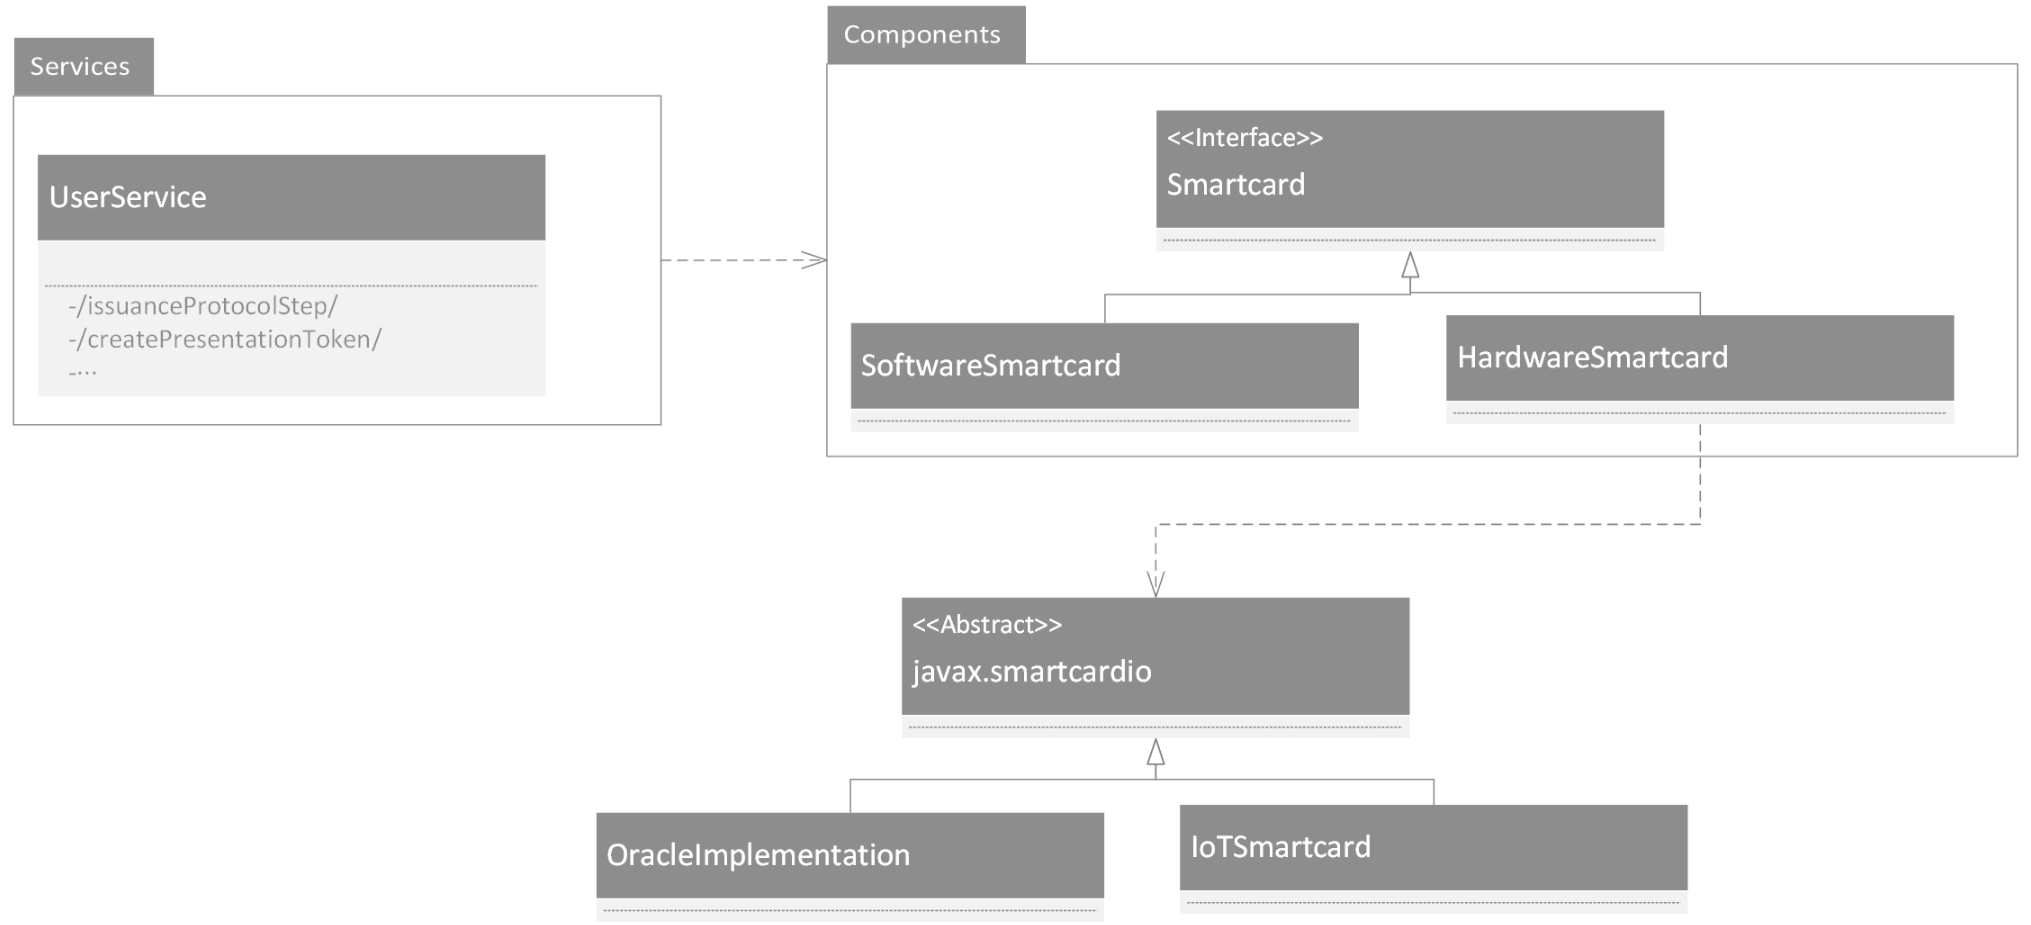
\includegraphics[width=\linewidth]{gfx/p2abceBasicUML}
	\end{center}
	\caption{Basic P2ABCE structure}
	\label{fig:p2abceBasicUML}
\end{figure}


As a PoC the P2ABCE project includes the ABC4Trust Card Lite, an implementation for ML3-36K-R1 Multos Smartcards. The code is written in C, but is very dependent on the Multos framework, aside from numerous bugs and bad coding habits. 



At this stage, we have two options to implement our IoT device compatible with P2ABCE:

\begin{itemize}
	\item Implement in C the \textit{Smartcard} interface used by P2ABCE architecture, and use some communication protocol to remotelly call the methods from the machine running the P2ABC Engine.
	\item Present the IoT device as a hardware smart card, using the APDU protocol (already defined, standard and with minimal overload). Providing a \textit{javax.smartcardio} ``IoT implementation'' to communicate with the IoT device through a transmission protocol, the already existing \textit{HardwareSmartcard} class can work with the new \textit{IoTSmartcard} in the IoT device.
\end{itemize}



%TODO : hablar más de los servicios REST



\section{MULTOS}

MULTOS is a multi-application smart card operative system, which provides a custom developing environment, with rich documentation \citep{MultosTechLib}. MULTOS smart cards communicate like any other smart card following the standard, but internally offers a very specific architecture, affecting the way one must code applications for it.

In this section we will present the main characteristics of a MULTOS smart card that shaped the ABC4Trust Card Lite code and that we had to be aware of when adapting it to IoT devices.

\paragraph{MULTOS programming languages} A native assembly language called MEL, C and, to a lesser extent, Java, are the available languages to code for MULTOS. In our case, ABC4T Card Lite uses MEL and C.

\paragraph{MULTOS Workflow}

Most of the transmission and communication process is done by MULTOS core, and it then selects, based on the CLA byte of the APDU, the application to load. This application is what most developers will only worry about, and is where their $main()$ function will start.

\begin{figure}[bth]
	\begin{center}
		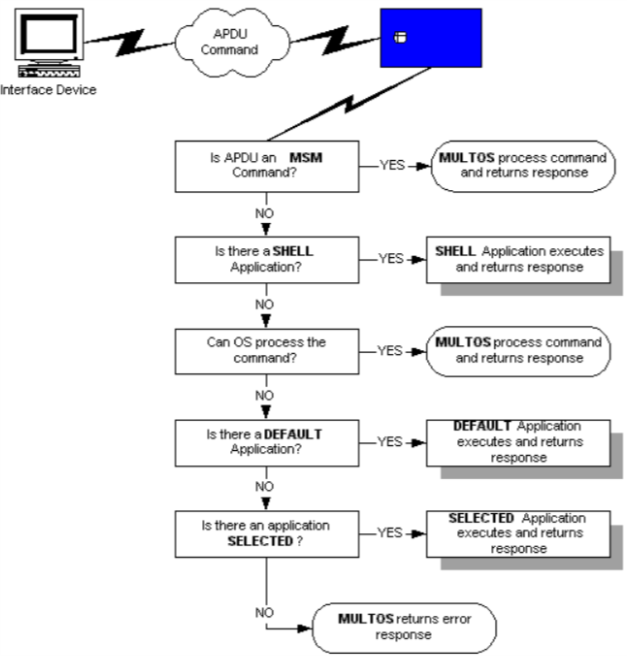
\includegraphics[width=\linewidth]{gfx/multosWorkflow}
	\end{center}
	\caption{MULTOS workflow}
	\label{fig:multosWorkflow}
\end{figure}

The application uses then the \textit{multos.h} file that declares multiple global variables already loaded with the needed data, including the APDU Command bytes.

Now the developer is in charge of checking what instruction was sent and if the APDU has the expected ISO Case. If everything is ok, code what needs to be run and write in specific data space the APDU Response bytes, call \textit{multosExit()} and MULTOS will be in charge to send the APDU Response.

In summary, our application starts with all data loaded and exits without worrying how to send the answer. A very comfortable workflow that we must now implement for our IoT device if we would want ABC4T Card Lite code to work.

\paragraph{MULTOS Memory Layout}

Each application in MULTOS has access to a specific memory layout, divided in different categories:

\begin{figure}[bth]
	\begin{center}
		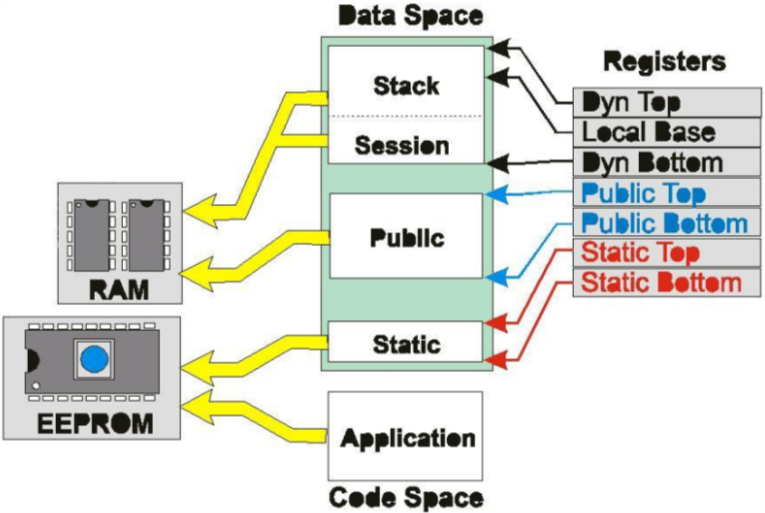
\includegraphics[width=\linewidth]{gfx/multosMemLay}
	\end{center}
	\caption{MULTOS Memory Layout}
	\label{fig:multosMemLay}
\end{figure}


The Code Space is where the application code is stored.
The Data Space is divided in Static memory, Public memory and Dynamic memory.

\textbf{Static memory} are the application variables declared after the specific \textit{\#pragma melstatic} compiler directive. These variables are stored in the non-volatile EEPROM, and any write is assured to be saved because they are not loaded into RAM.

\textbf{Public memory} can be seen as the input/output buffer for applications and MULTOS system. The APDU header appears at the top of Public, and command data at the bottom. The application writes then the APDU Response bytes in Public, at specific position (see \autoref{fig:multosPubMem}). To declare variables in this data space, the \textit{\#pragma melpublic} directive is available.

\textbf{Dynamic memory} works like usual program memory, with Session Data storing global variables and the Stack. The limited size of RAM in IoT devices and smart cards makes the use of dynamic memory not advisable. The compiler directive to use Session Data is \textit{\#pragma melsession}.


\begin{figure}[bth]
	\begin{center}
		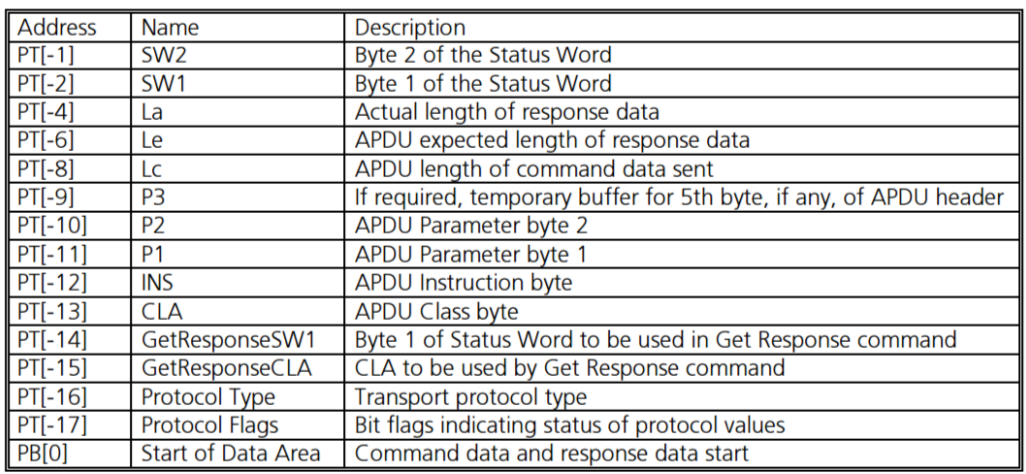
\includegraphics[width=\linewidth]{gfx/multosPubMem}
	\end{center}
	\caption{MULTOS Public Memory Data Map}
	\label{fig:multosPubMem}
\end{figure}


\hfil


With regards to primitive types, to avoid confusion with their sizes, MULTOS defines and uses the following data types specified in \autoref{fig:multosDataTypes}. It's important to notice that MULTOS is Big Endian
\marginpar{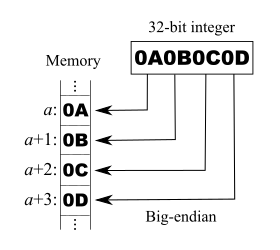
\includegraphics[width=\linewidth]{gfx/Big-Endian}\\Big-Endian, Wikipedia}
and when storing structures there is no padding between defined variables, unlike modern compilers that perform data structure alignment \citep{dataStructAlign} for performance.

\begin{figure}[bth]
	\begin{center}
		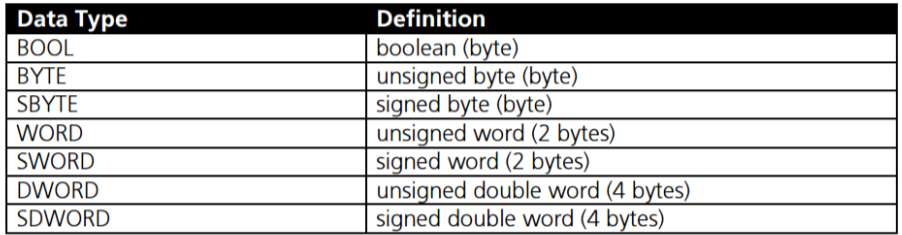
\includegraphics[width=\linewidth]{gfx/multosDataTypes}
	\end{center}
	\caption{MULTOS Data Types}
	\label{fig:multosDataTypes}
\end{figure}


\paragraph{MULTOS Standard C-API}

A collection of more than a hundred functions are provided for arithmetic, cryptography, memory and smart card operations. The \textit{multos.h} interface provides access to these functions, that ultimately call their respective primitive instructions in assembly code. The primitive instructions are but a system call with an operation code, loading data in the needed registers. Therefore,  no implementation for these tools is available, nor in C, nor in assembly code.

Nevertheless, the C-API documentation \citep{MultosTechLib} provides rich description for each function.





\section{ABC4Trust Card Lite}

The code from the P2ABCE project for a MULTOS smart card has some good and bad points to have in count:

The best asset of this code is that it's written in C aiming to a very constrained device, similar in computational power to typical IoT devices, and very limited memory.
	
Some \textit{tricks} include using \textit{union} for data types that will be stored on the same data location, but at different moments (e.g. depending on APDU Command INS byte) or strong use of pointers and \textit{memcpy} calls to copy \textit{structs} with multiple variables as arrays of bytes.


Among the many drawbacks we could mention the awful coding, the dependency on MULTOS framework and bugs. 

The code is structured in two files, \textit{main.h} and \textit{main.c}, with 557 and 5157 lines of code respectively.

The file \textit{main.h} is mostly a reimplementation in assembly MEL of some MULTOS' C-API functions available in \textit{multos.h}.

The \textit{main.c} consists on near 600 lines of variables and data structures declarations, followed by the \textit{main()} function, a 2635 lines long \textit{switch-case} with practically no comments, to conclude with the implementation of thirty functions called \textit{Subroutines} at the end of the file.


This gives an idea of the problematic to maintain or even understand the code. But once one studies MULTOS framework and applies many refactoring techniques to ABC4T Card's code, this becomes the best starting point for the IoT version.





\section{IoT smart card code}

After many design decisions in the process to adapt the original ABC4T Card Lite code to pure C over an standard architecture machine, in this section we present the current PoC code, most important decisions, workflow, and future work.


















\section{IoT and P2ABCE}

In this section we will define how an IoT device will be integrated in the P2ABCE environment, being totally compatible with any other system using P2ABCE, addressing the power and memory constrains IoT devices face.


\hfil

Our main goal is to make an IoT device capable to act as an User or Verifier in the P2ABCE architecture. For this, the device should manage complex XML schemas, perform cryptographic ZKP operations and communicate with the Verifier or Prover with which it's interacting.

The communication is already solved by the \textit{Internet} capabilities of IoT devices.

Our concern are the XML files exchanged and the cryptographic operations involving secret keys that must remain private to the IoT device.

Here is where we look at the P2ABCE architecture more closely, and the concept of smart cards shows a solution for the second issue. Even in the case we were to implement all P2ABCE inside an IoT device, we would have to implement support for software smart cards, to keep the secret inside the IoT device. We will start building the house from the ground, implementing the smart card operations inside the IoT device.

Now that in our design we have the smart card, we need to address the first point, XML data. %TODO